\documentclass[11pt]{article}
\usepackage{graphicx}
\usepackage[margin=0.75in]{geometry}

\graphicspath{ {image/} }

\title{Classification of fMRI Data}
\author{
  Chang, Zheng\\
  \texttt{changzheng1993}
  \and
  Escobar, Giancarlo\\
  \texttt{giancarloescobar}
  \and
  Pimentel, Noel\\
  \texttt{noelpimentel}
  \and
  Yousuf, Imran\\
  \texttt{imranyousu}
}

\bibliographystyle{siam}

\begin{document}
\maketitle

\abstract{The functional architecture of the object vision pathway in the human brain was 
investigated using fMRI imaging to measure patterns of response in ventral 
temporal cortex while subjects viewed categories of objects in Haxby et al. 
[Science 293 (2001) 2425] \cite {haxby2001vt}. Haxby argued that 
category related responses in the 
VT lobe during visual object identification were overlapping and distributed in 
topography. At the time of Hanson et al. [Elsevier 23 (2004) 156] \cite 
{hanson2004combinatorial} there were prevailing views that objects codes were 
focal and localized to specific areas like the fusiform and the parahippocampal 
gyri.  Hanson et al. revisited the Haxby data and provided a crucial test of 
the former hypothesis using a neural network classifier.  The method of Hanson 
et al. detected more general topographic representations and illustrated that 
substantially the same VT lobe voxels contribute to classification of all 
object categories
}

\section{Introduction}

\setlength{\parskip}{10pt}

Models for the functional architecture of the ventral temporal cortex fall into 
three categories. One model proposes that VT contains a limited number of areas 
that are specialized for representing specific categories of stimuli. A second 
model proposes that different areas in VT are specialized for different types 
of perceptual processes. The third model proposes that the representations of 
faces and different categories of objects are widely distributed and 
overlapping.  According to the latter model, VT has a topographically organized 
representation of attributes of form that underlie face and object recognition 
meaning that the representation of a face or object is illustrated by a unique 
pattern of response across a wide expanse of cortex in which primary and 
secondary regions (i.e. large- and small-amplitude responses) hold information 
about face and object appearance.

Haxby et al. tested this model by investigating the patterns of response evoked 
in the ventral temporal cortex by faces and multiple categories of objects 
(face, house, cat, bottle, scissors, shoe, chair, scrambled image) in a series 
of runs on six subjects. Patterns of response were defined as those voxels with 
response that differed significantly by category and will be referred to as POR 
for future purposes. The data \cite{haxby2001vor} were analyzed to determine 
whether the stimulus category that a subject was viewing could be identified on 
examining the similarity between the POR evoked by each category on even and 
odd runs. Within-category correlations and between-category correlations were 
compared to determine whether a POR to one category, such as chairs, could be 
distinguished from the pattern of response to a different category, such as 
shoes, with and without the exclusion of maximally responsive voxels. For the 
inclusion of maximally responsive voxels, The POR in object-selective ventral 
temporal cortex correctly identified the category being viewed in 96 percent of 
pairwise comparisons. Identification accuracy for faces, houses, and scrambled 
pictures was at 100 percent and identification accuracy for the small man-made 
objects (bottles, scissors, shoes, and chairs) was significantly better than 
chance for each category. For the exclusion of maximally responsive voxels, for 
example, within the cortex that responded maximally to houses, the POR 
correctly identified the category being viewed with 93 percent accuracy, 94 
percent for small man made objects, and 83 percent for faces.  These results 
demonstrate that POR in VT carries information about the type of object being 
viewed, even in cortex that responds maximally to other categories.

The work by Hanson et al. established Haxby et al. results while further 
extending the original analysis.  Hanson et al. neural network classifier 
detected more general topographic representations and achieves an 83 percent 
correct generalization performance on patterns of voxel response in 
out-of-sample tests.  Using voxel-wise analysis Hanson et al. showed that the 
same VT lobe voxels contribute to the classification of all object categories, 
suggesting that the code is combinatorial as Haxby et al. suggested. Our own 
analysis will adhere to the methods of Haxby et al. and Hanson et al. with the 
plan of reproducing the Haxby similarity method (comparisons between 
within-category correlation and between-category correlation) and reproducing 
and improving upon the POR classification rate with a neural network and 
homogenous methods. We will make the these studies reproducible in the sense 
that code used to obtain said results will be easily understandable and 
readable by others; any graph, statistics, etc. from these studies can be 
easily simplified and reproduced with the aid of well documented executable and 
readable code.

\section{Data}

The data consists of 64 slices  64 X 40 BOLD collected from a GE 3T (repetition 
time = 2500 ms, forty 3.5-mm-thick sagittal images, field view of = 24 cm, echo 
time = 30 ms, flip angle = 90 percent). Patterns of neural response were 
measured with functional magnetic resonance imaging (fMRI) in six subjects 
while they viewed pictures of faces, cats, five categories of manmade objects. 
Twelve time series were obtained for each subject. Each time series began and 
ended with 12-s rests and contained eight stimulus blocks of 24-s duration, one 
for each category, separated by 12-s interval of rest. Stimuli were presented 
for 500 ms with an inter stimulus interval of 1500 ms. Repetitions of 
meaningful stimuli were pictures of the same face or object photographed from 
different angles; stimuli for each meaningful category were four images each of 
12 different exemplars. The data shape for any particular run is (40, 64, 64, 
121) that can be read as 64 slices 64 X 40 BOLD for 121 contiguous slices in 
time (i.e. 121 volumes of time).


\section{Methods}

\subsection{Preprocessing/ EDA}

The Haxby data consists of six folders for each individual subject. Each of 
these folders contains the fMRI data along within 12 folders, one for each run. 
 The structure of the data is cumbersome and for reasons of reproducibility, 
and for our own sake, we implemented code to merge these 12 runs by calling on 
a function and passing through the argument of subject name (i.e. 'sub001', 
'sub002',..., 'sub012').  This code conveniently merges the 12 runs for any 
specified subject. fMRI can have a considerable degree of noise. There are 
often volumes with an unusual degree of noise and for that reason these volumes 
can produce outliers in voxel time-courses. Another sign of an artifact in a 
volume is that a given volume is very different from the preceding volume. This 
would imply a sudden wide-spread shift in signal. 

We calculated the standard deviation of every volume, 121x12 = 1452 volumes, 
for each subject and identified outliers with two methods. The first method was 
the interquartile range which is the value of the 75th percentile minus the 
25th percentile. We might decide to declare a value as an outlier, if the value 
(i.e. voxel standard deviation) is greater than 1.5 * IQR added to the 75th 
percentile, or lower than 1.5 * IQR subtracted from the 25th percentile. The 
second method assesses outliers by taking the square root of the mean of the 
squared voxel values where these voxel values correspond to the difference of a 
subject's 3D volume from the subsequent volume. The interquartile range method 
is applied to these values to obtain outliers.

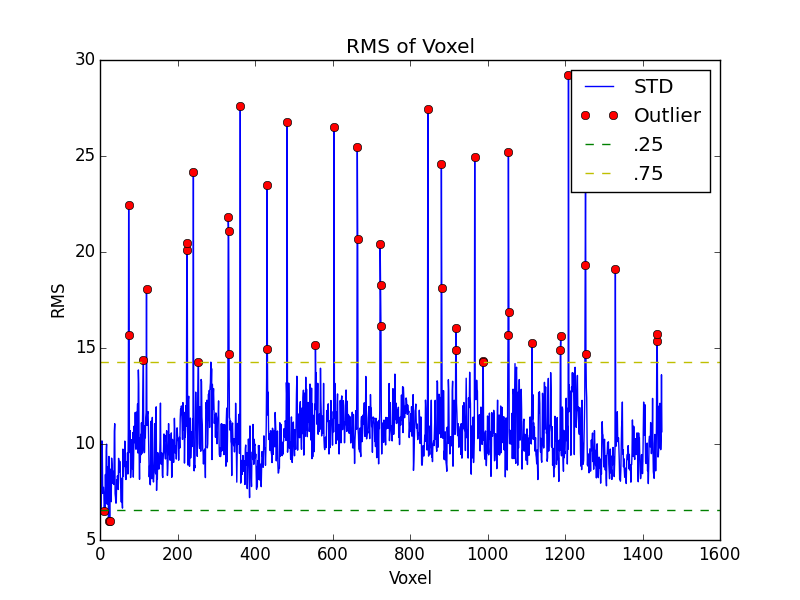
\includegraphics[scale=0.75]{vol_rms_outliers.png}

If we have done a good job of identifying and removing outliers, we would 
expect a drop in the residuals from a statistical model (e.g. linear model).


\section{Results}

\subsection{Discussion}

Most of our analysis consisted of exploring the structure of our data, 
comprehending the analysis of Haxby et al. and Hanson et al., and formulating 
and setting up major groundwork for the reproducibility aspect of our code for 
analysis. This left us with some time to preprocess the data by performing 
simple outlier identification; we also performed some rough convolution which 
needs some touching up. The scikit-learn package for machine leaning package we 
wish to use on the data requires a merging of a subjects 12 runs of data.  A 
good amount of time was spent on merging the data and in understanding the ways 
of the package.  The Git workflow further extended this time as those 
unfamiliar to the workflow practiced to become familiarized to it.  The 
structure and study of the fMRI data itself is something new and unfamiliar 
territory; therefore, we made it a priority to understand the basics of 
previous analyses and structures of our data.  Our future work will contain 
more analysis, for we are set to begin. In our next step we will reduce the 
dimension of our data (i.e. perform PCA or PLR), we will then produce a sparse 
model (i.e. perform ridge/lasso and cross validation to identify crucial voxels 
and appropriate tuning parameters), and determine the best way to split our 
data (i.e. perform cross validation on different statistical models). 


\bibliography{project}

\end{document}
